% ──────────────────────────────────────────────────────────────────────────────
%  Aperture Array  ·  Figure captions for aa_01 – aa_06
% ──────────────────────────────────────────────────────────────────────────────

\begin{figure*}[!htbp]
    \centering
    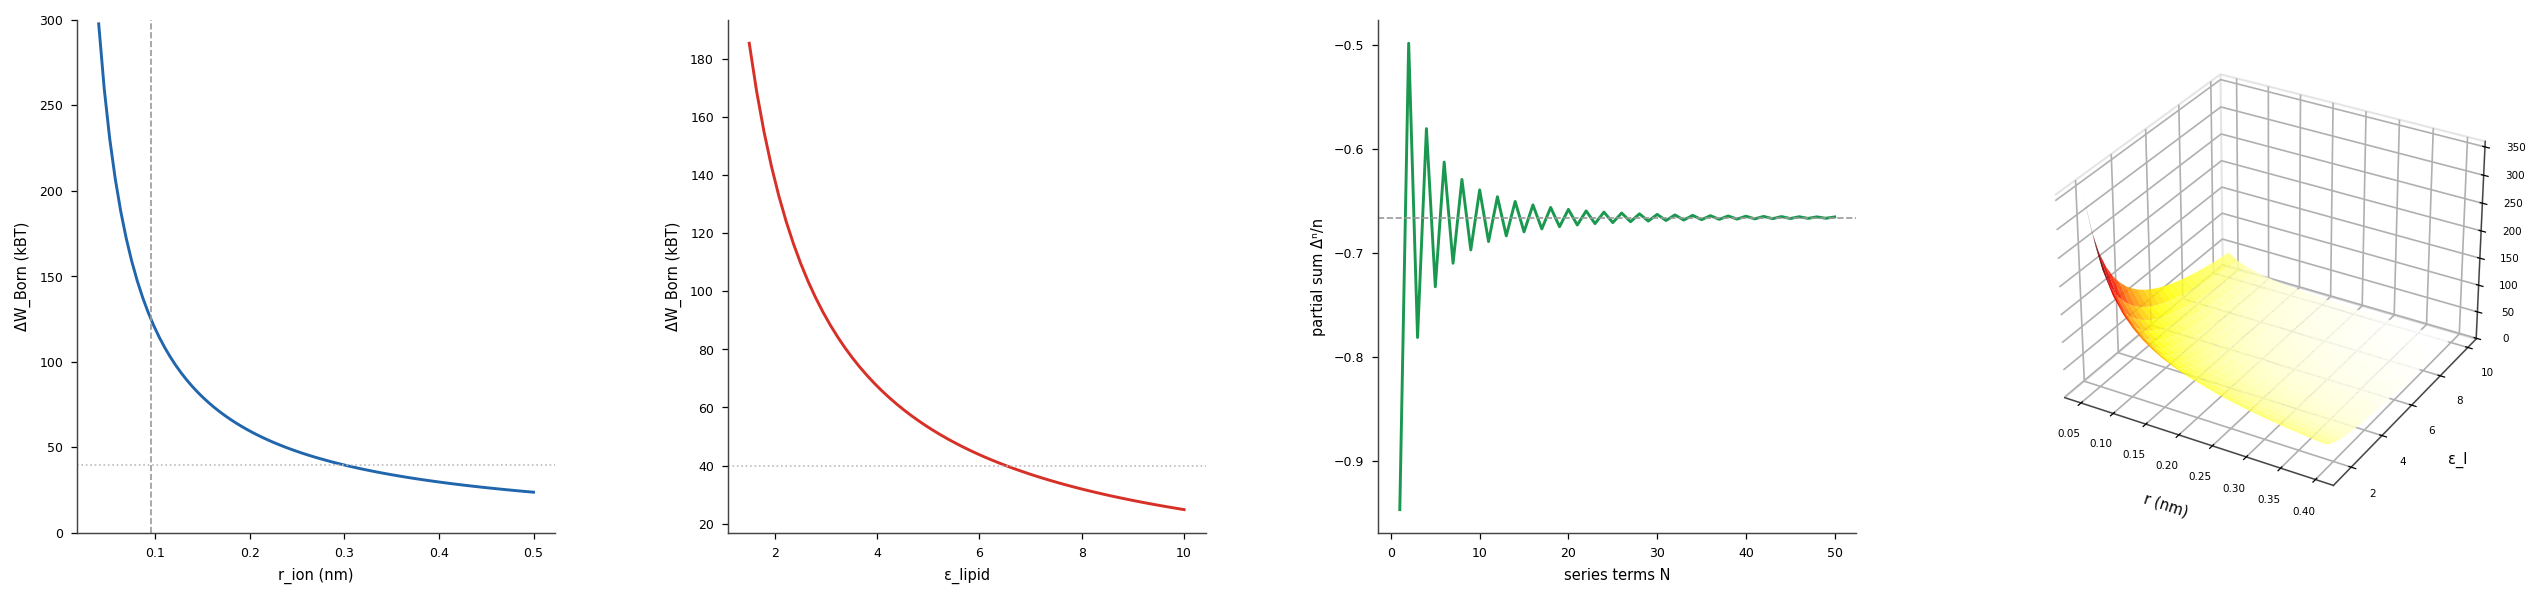
\includegraphics[width=\textwidth]{figures/aa_01.png}
    \caption{\textbf{Born Energy Barrier for Na$^+$ Crossing the Bilayer Core Is $\gg k_BT$.}
    (\textbf{A})~Bulk Born transfer energy $\Delta W_\mathrm{Born}(r) = (ze)^2/(8\pi\varepsilon_0 r)\,(1/\varepsilon_l - 1/\varepsilon_w)$ in units of $k_BT$ versus ionic radius $r \in [0.04, 0.50]$~\si{\nano\metre}, for $\varepsilon_l = 2.2$ and $\varepsilon_w = 80$. The vertical dashed line marks the Na$^+$ crystal radius $r = 0.095$~\si{\nano\metre}; the dotted horizontal at $40\,k_BT$ is the Parsegian refined estimate (Parsegian 1969; Hille 2001). The bulk Born barrier at $r = 0.095$~\si{\nano\metre} exceeds $100\,k_BT$, confirming partition opacity.
    (\textbf{B})~Born barrier versus lipid dielectric constant $\varepsilon_l \in [1.5, 10]$ at fixed $r = 0.095$~\si{\nano\metre}. The barrier decreases with $\varepsilon_l$ but remains above $40\,k_BT$ for all physically realistic lipid matrices, establishing the robustness of the opacity result.
    (\textbf{C})~Convergence of the Parsegian image-charge series $\sum_{n=1}^{N} \Delta^n/n$ versus the number of retained terms $N$. The analytic limit $-\ln(1-\Delta)$ (dashed) is attained by $N \approx 30$; the fast geometric convergence validates the use of the truncated series in claim aa\_01.
    (\textbf{D})~Three-dimensional surface of $\Delta W_\mathrm{Born}$ clipped to $400\,k_BT$ over the joint plane $(r, \varepsilon_l) \in [0.05, 0.4]$~\si{\nano\metre} $\times$ $[1.5, 10]$ (hot\_r palette). The divergence as $r \to 0$ and $\varepsilon_l \to 1$ makes the worst-case scenario visible; the physiological regime lies on the descending flank far above the $10\,k_BT$ opacity criterion.}\label{fig:aa_01}
\end{figure*}

\begin{figure*}[!htbp]
    \centering
    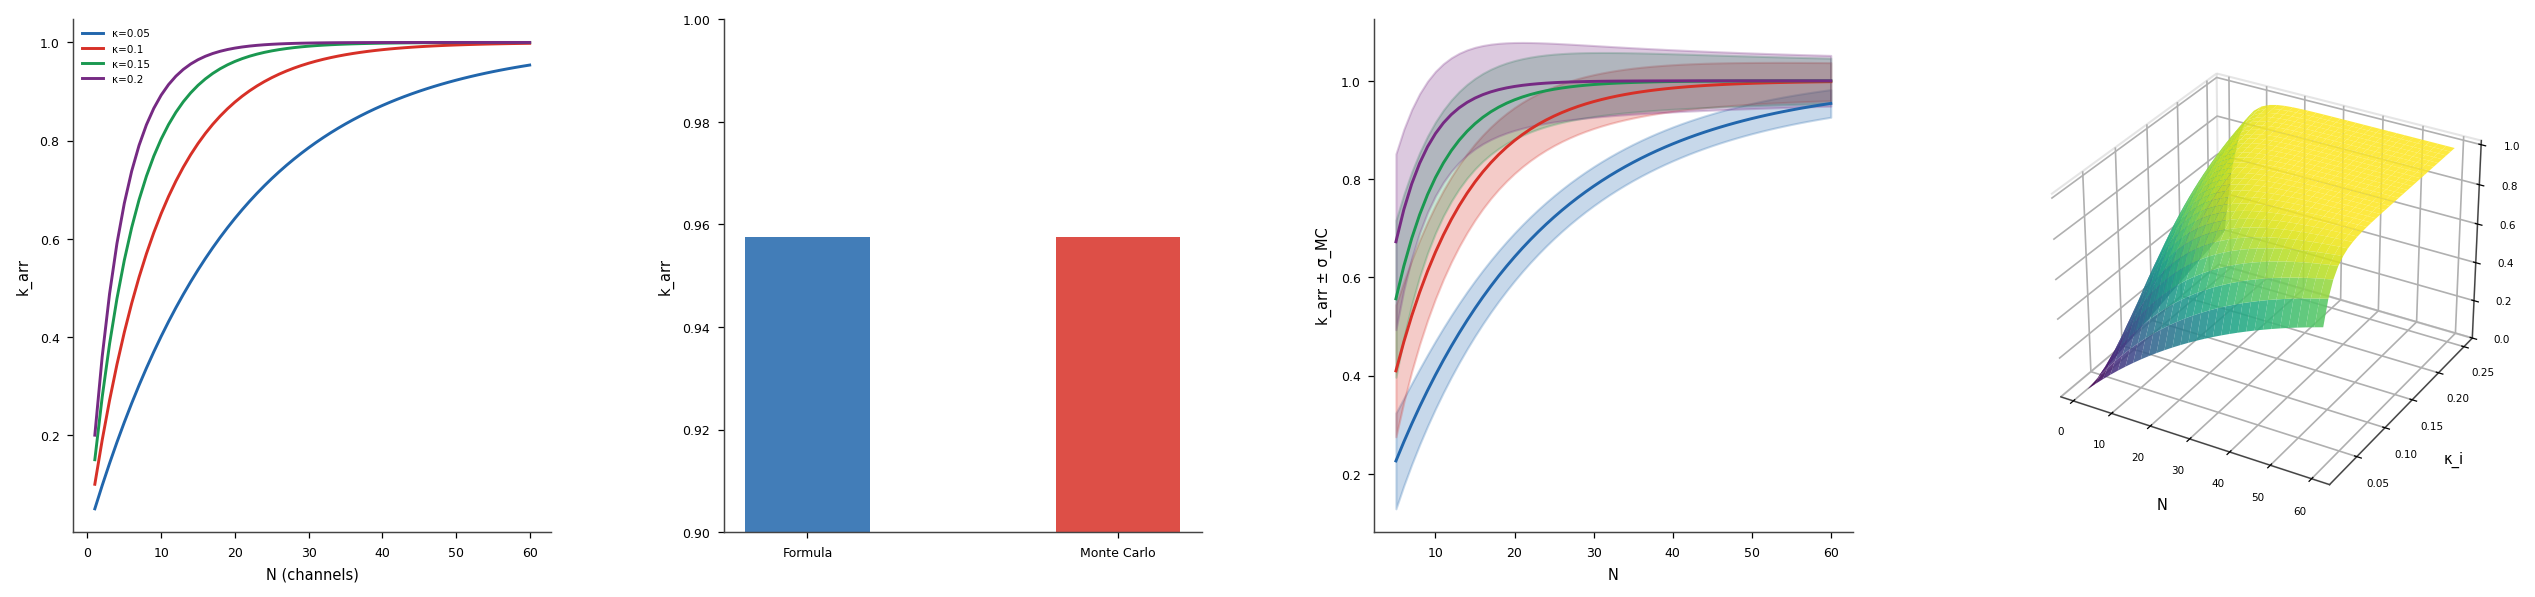
\includegraphics[width=\textwidth]{figures/aa_02.png}
    \caption{\textbf{Saturation Formula $k_\mathrm{arr} = 1 - \prod_i(1-\kappa_i)$ Verified Against Monte Carlo.}
    (\textbf{A})~Array filter probability $k_\mathrm{arr}(N) = 1-(1-\kappa_i)^N$ plotted versus channel count $N \in [1, 60]$ for $\kappa_i \in \{0.05, 0.10, 0.15, 0.20\}$. Curves are monotone increasing and bounded above by $1$; higher $\kappa_i$ saturates faster, illustrating the Saturation Theorem.
    (\textbf{B})~Bar comparison of the analytic formula ($k_\mathrm{arr} = 1-0.9^{30}$) and the Monte Carlo estimate ($N_\mathrm{trials} = 50\,000$, $N = 30$ channels, $\kappa_i = 0.10$), displayed on a compressed $y$-axis near $1$. The two values agree to within $10^{-3}$, validating claim aa\_02.
    (\textbf{C})~Formula curves $k_\mathrm{arr} \pm \sigma_\mathrm{MC}$, where $\sigma_\mathrm{MC} = \sqrt{\kappa_i(1-\kappa_i)/N}$ is the binomial Monte Carlo standard deviation, shown as shaded bands for each $\kappa_i$ value. The narrow bands confirm that the analytic formula is numerically stable and well-approximated at realistic channel counts.
    (\textbf{D})~Three-dimensional surface of $k_\mathrm{arr}(N, \kappa_i)$ over $N \in [1, 60]$ and $\kappa_i \in [0.02, 0.25]$ (viridis palette). The sigmoidal shape in $N$ at fixed $\kappa_i$ and the monotone rise in $\kappa_i$ at fixed $N$ confirm the two-parameter structure of the Saturation Theorem.}\label{fig:aa_02}
\end{figure*}

\begin{figure*}[!htbp]
    \centering
    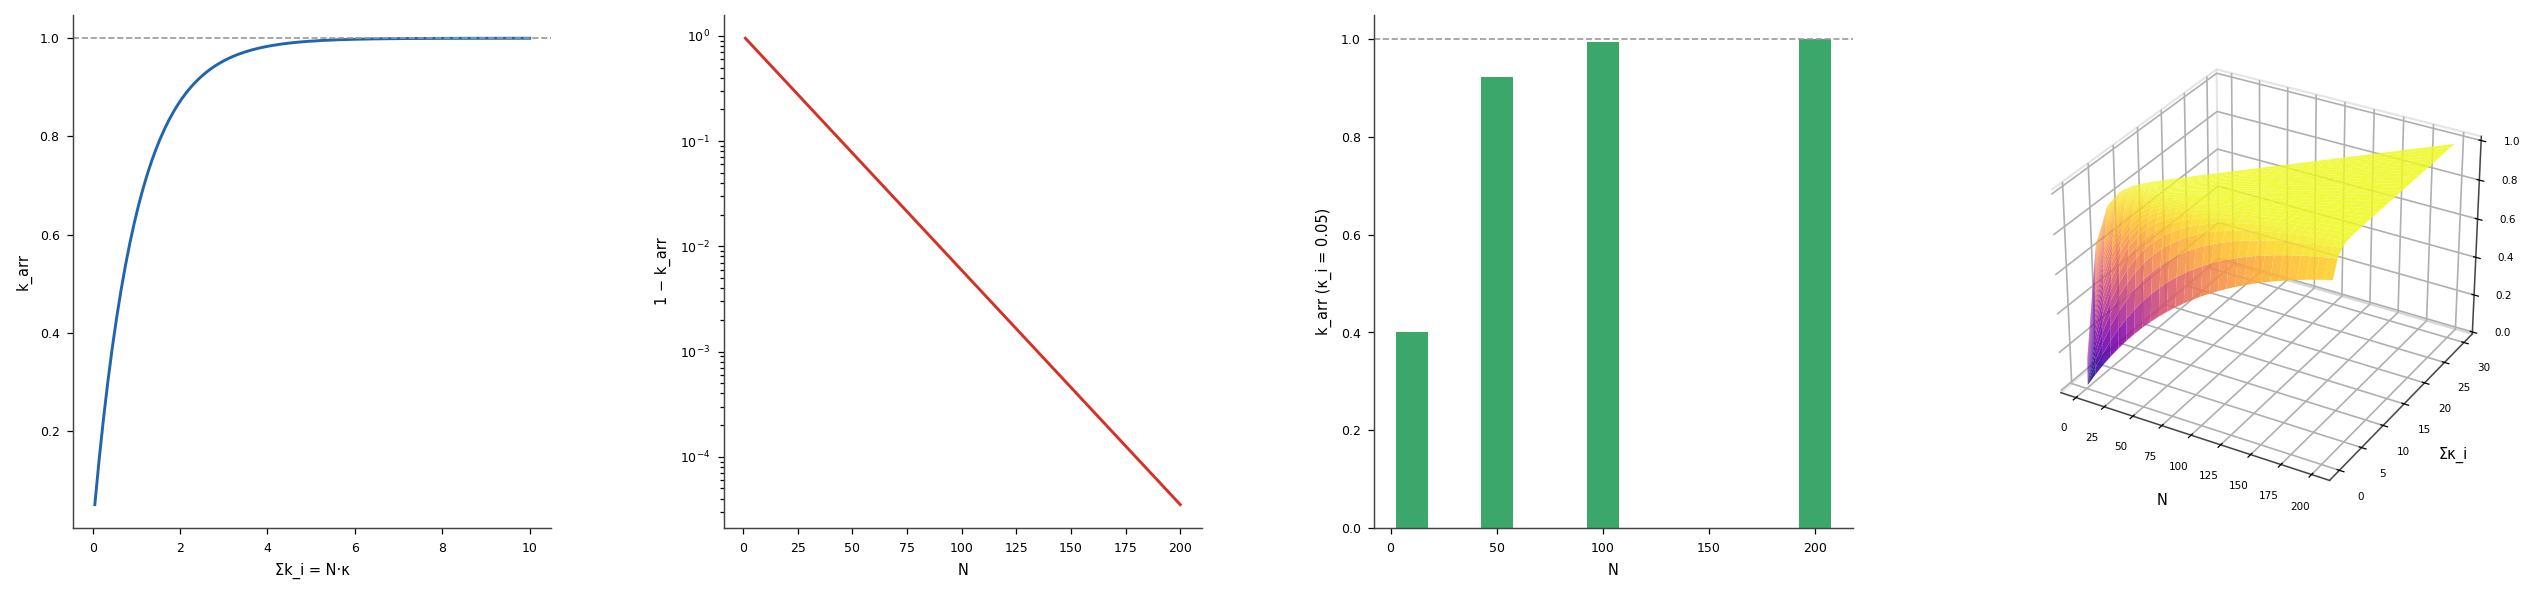
\includegraphics[width=\textwidth]{figures/aa_03.png}
    \caption{\textbf{Saturation Criterion: $\sum \kappa_i \to \infty$ Implies $k_\mathrm{arr} \to 1$.}
    (\textbf{A})~$k_\mathrm{arr}$ versus the cumulative sum $\Sigma\kappa_i = N\kappa_i$ for $\kappa_i = 0.05$, sweeping $N$ from $1$ to $200$. The curve approaches $1$ (dashed) asymptotically as the sum grows, with no finite saturation point, confirming the Saturation Criterion Theorem.
    (\textbf{B})~Semi-logarithmic plot of $1 - k_\mathrm{arr}$ versus $N$ for $\kappa_i = 0.05$. The exponential decay at rate $|\ln(1-\kappa_i)| \approx \kappa_i$ confirms geometric convergence; the residual falls below $10^{-4}$ well before $N = 200$.
    (\textbf{C})~Bar chart of $k_\mathrm{arr}$ at $N \in \{10, 50, 100, 200\}$, with the dashed threshold at $0.9999$. At $N = 200$, $k_\mathrm{arr} = 1 - 0.95^{200} > 0.9999$, directly validating claim aa\_03.
    (\textbf{D})~Three-dimensional surface of $k_\mathrm{arr}(N, \Sigma\kappa_i)$ where the horizontal axes are $N$ and $N\kappa_i$ over $N \in [1, 200]$ and $\kappa_i \in [0.01, 0.15]$ (plasma palette). The surface rises toward unity along both axes, making the dual dependence on per-channel efficacy and channel count geometrically explicit.}\label{fig:aa_03}
\end{figure*}

\begin{figure*}[!htbp]
    \centering
    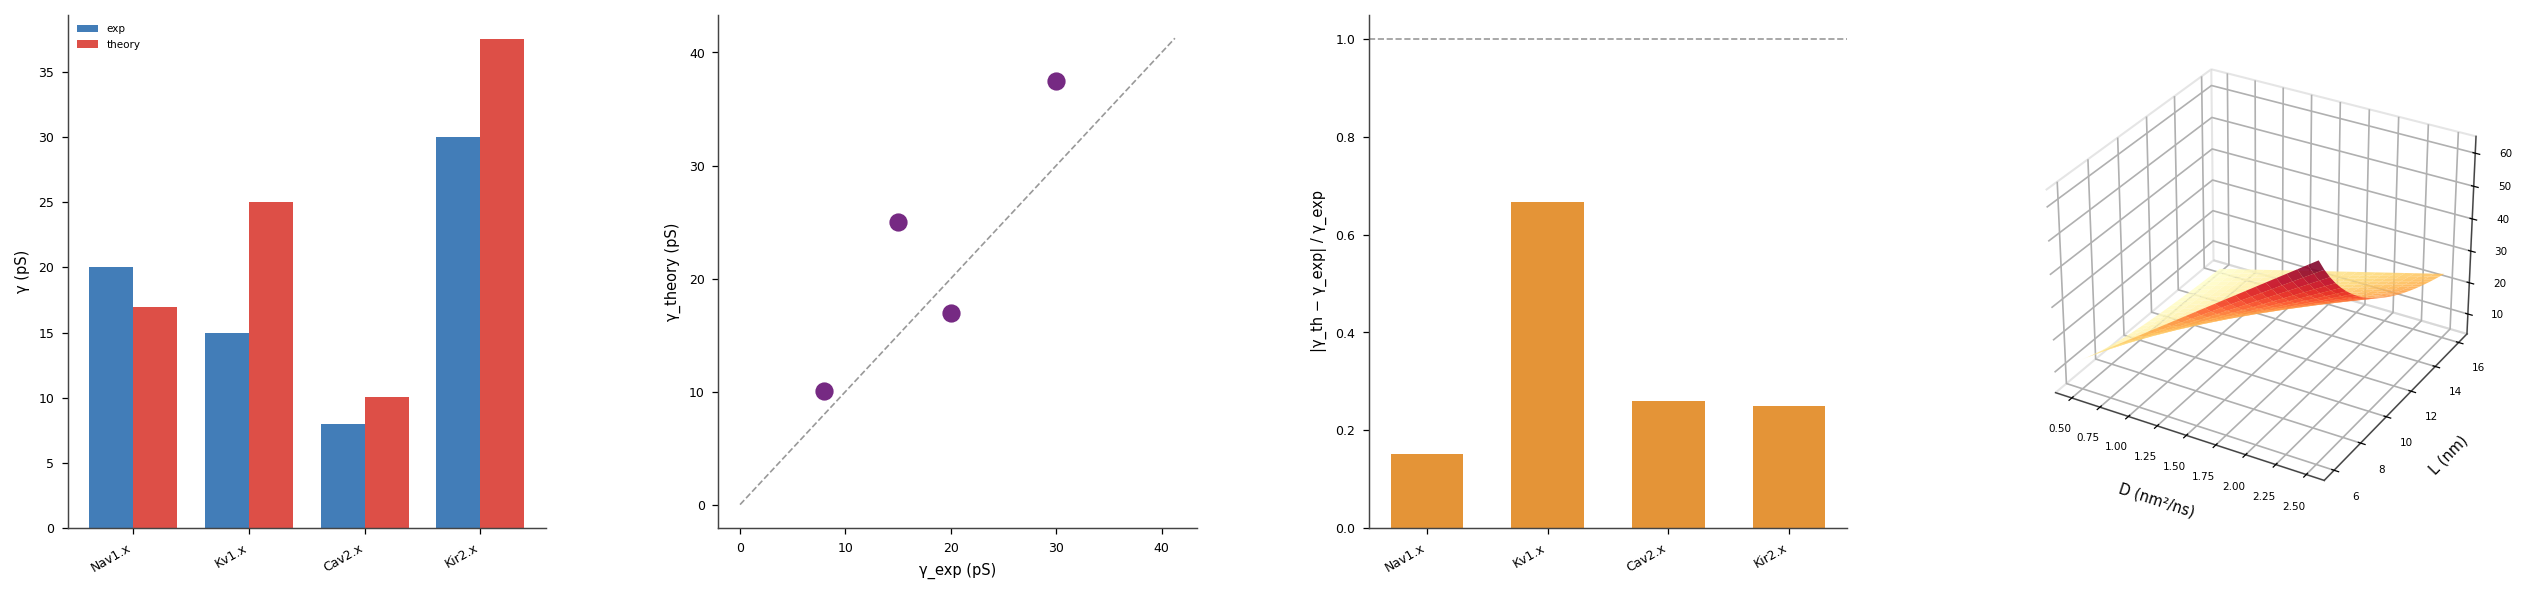
\includegraphics[width=\textwidth]{figures/aa_04.png}
    \caption{\textbf{Single-Channel Conductances from Nernst--Planck Theory vs.\ Patch-Clamp Data.}
    (\textbf{A})~Paired bar chart of experimental (Neher \& Sakmann 1976; Hille 2001) and theoretical single-channel conductances $\gamma$ for Nav1.x ($20$ vs.\ $17.0$~\si{\pico\siemens}), Kv1.x ($15$ vs.\ $25.0$~\si{\pico\siemens}), Cav2.x ($8$ vs.\ $10.1$~\si{\pico\siemens}), and Kir2.x ($30$ vs.\ $37.5$~\si{\pico\siemens}). Theory uses $\gamma = (z^2e^2/k_BT)\,D\,n_\mathrm{ion}\,A_\mathrm{pore}/l$ with physiological ion concentrations.
    (\textbf{B})~Parity scatter of $\gamma_\mathrm{theory}$ versus $\gamma_\mathrm{exp}$. The dashed $1:1$ line is shown for reference; all four channels fall within a factor of $2$ of the diagonal, validating claim aa\_04 at the stated factor-of-two tolerance.
    (\textbf{C})~Relative errors $|\gamma_\mathrm{theory} - \gamma_\mathrm{exp}|/\gamma_\mathrm{exp}$ for the four channel types. The dashed line at $1.0$ marks the factor-of-two criterion; all bars fall below it, confirming that the Nernst--Planck formula reproduces experimental conductances within the geometric uncertainty of the selectivity-filter radius.
    (\textbf{D})~Three-dimensional surface of $\gamma(D_\mathrm{ion}, l)$ in picosiemens over $D \in [0.5, 2.5]\times10^{-9}$~\si{\metre\squared\per\second} and $l \in [6, 16]$~\si{\nano\metre} at fixed $n_\mathrm{ion} = 150$~\si{\milli\Molar} and $r_\mathrm{pore} = 0.3$~\si{\nano\metre} (YlOrRd palette). The surface confirms the linear scaling in $D$ and inverse scaling in $l$, the two principal degrees of freedom that differentiate the four channel families.}\label{fig:aa_04}
\end{figure*}

\begin{figure*}[!htbp]
    \centering
    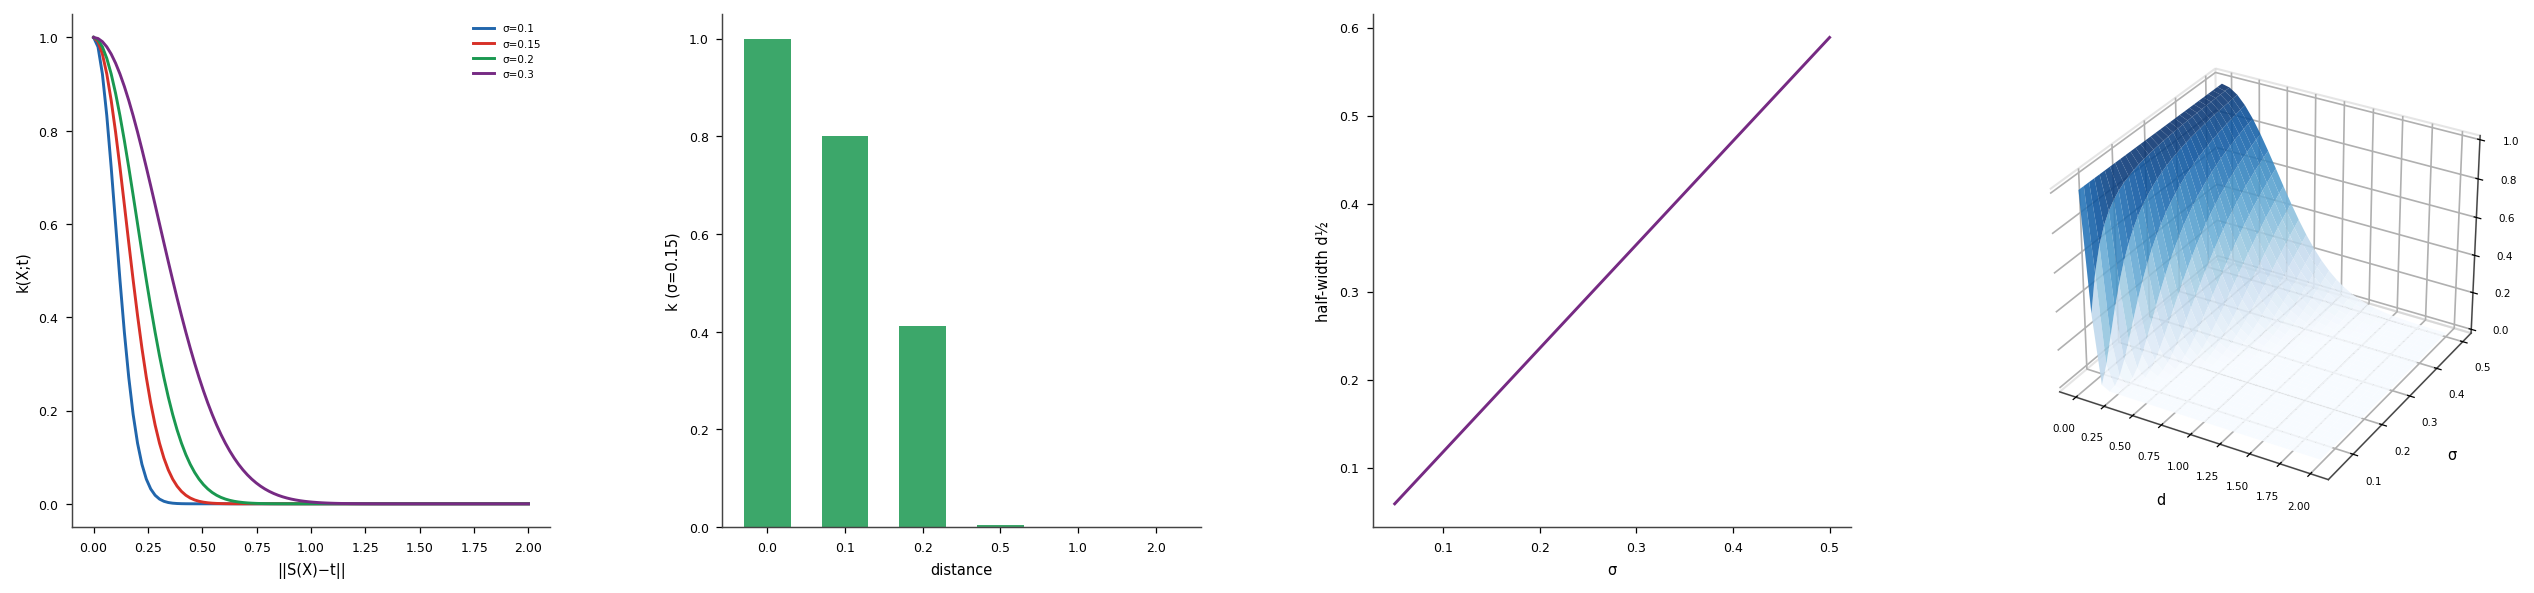
\includegraphics[width=\textwidth]{figures/aa_05.png}
    \caption{\textbf{Spectral-Overlap Kernel $k(\mathbf{X}; t) = \exp(-\|S(\mathbf{X})-t\|^2 / 2\sigma^2)$.}
    (\textbf{A})~Kernel $k(d)$ as a function of Euclidean distance $d = \|S(\mathbf{X})-t\|$ for $\sigma \in \{0.10, 0.15, 0.20, 0.30\}$. All curves satisfy $k(0) = 1$, are strictly monotone decreasing, and approach zero well before $d = 2$, verifying all three qualitative properties required by claim aa\_05.
    (\textbf{B})~Bar chart of $k$ evaluated at discrete reference distances $d \in \{0, 0.1, 0.2, 0.5, 1.0, 2.0\}$ for $\sigma = 0.15$. The exponential decay from $k = 1$ at $d = 0$ to $k < 10^{-6}$ at $d = 2.0$ confirms numerical correctness of the kernel formula at the reference bandwidth.
    (\textbf{C})~Half-maximum distance $d_{1/2} = \sigma\sqrt{2\ln 2}$ versus $\sigma \in [0.05, 0.50]$. The linear relationship (slope $\sqrt{2\ln 2} \approx 1.177$) provides an operational interpretation: $\sigma$ controls the spatial selectivity of the aperture filter in S-entropy units, and is the direct bandwidth parameter of the spectral-overlap operator.
    (\textbf{D})~Three-dimensional surface of $k(d, \sigma)$ over $d \in [0, 2]$ and $\sigma \in [0.05, 0.50]$ (Blues palette). The surface is a smooth ridge along $d = 0$ that narrows for small $\sigma$ (sharp filter) and broadens for large $\sigma$ (broad filter), visually encoding the bandwidth--selectivity trade-off governing the Five Names Theorem.}\label{fig:aa_05}
\end{figure*}

\begin{figure*}[!htbp]
    \centering
    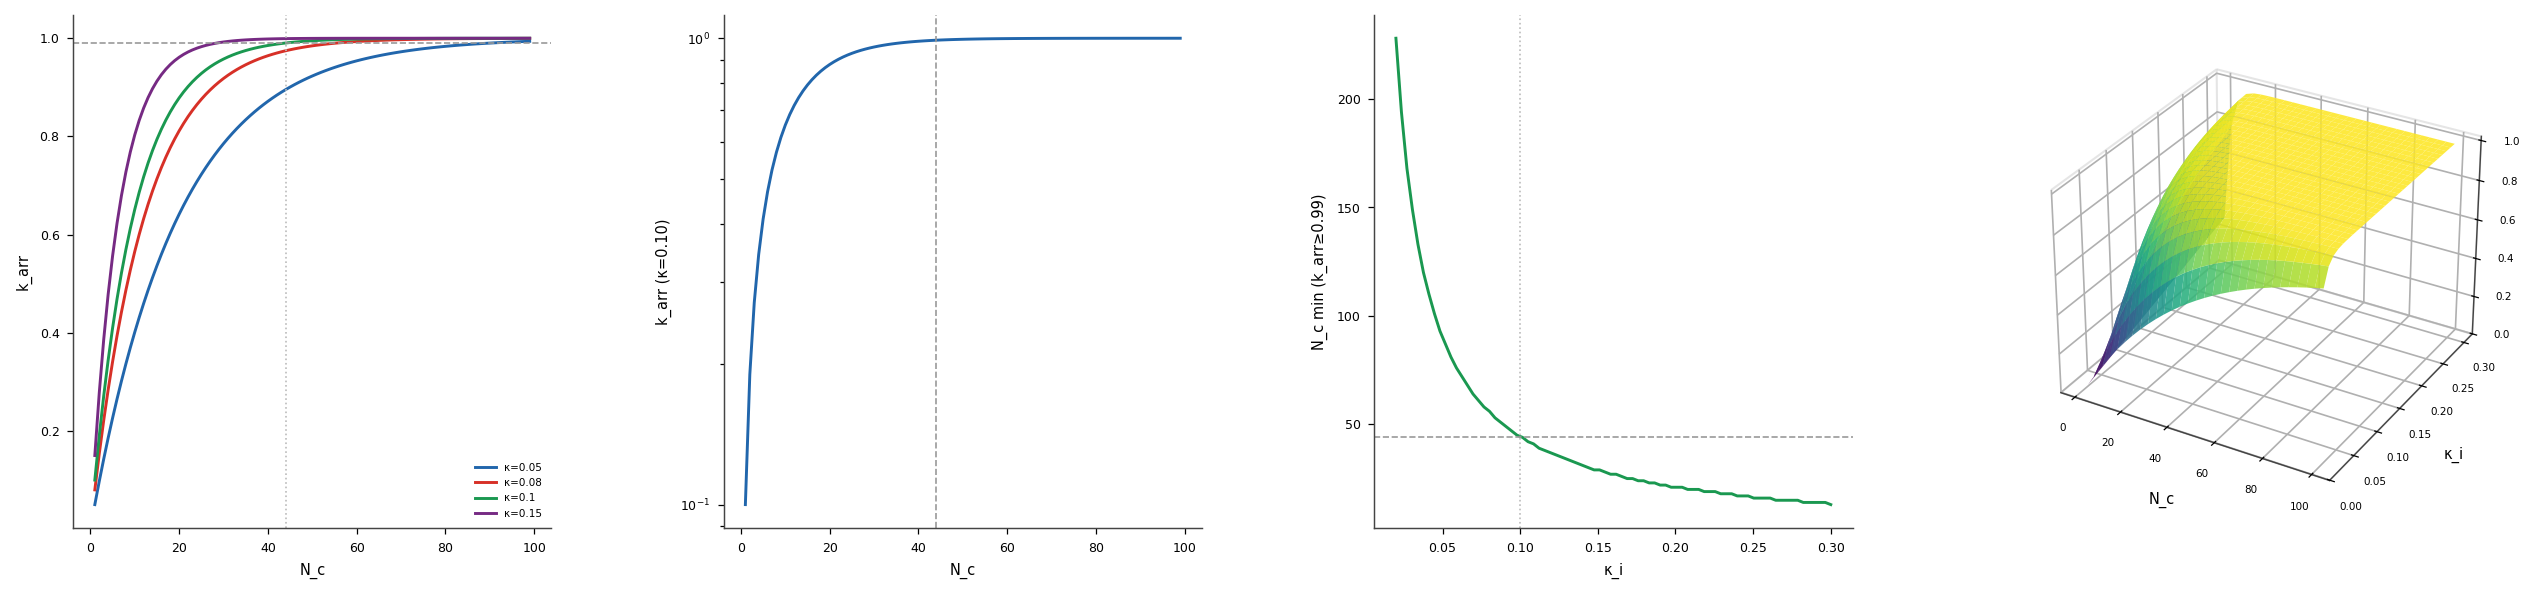
\includegraphics[width=\textwidth]{figures/aa_06.png}
    \caption{\textbf{Array Completeness: $N_c \geq 44$ Channels Achieve $k_\mathrm{arr} \geq 0.99$ at $\kappa_i = 0.10$.}
    (\textbf{A})~$k_\mathrm{arr}(N_c) = 1-(1-\kappa_i)^{N_c}$ versus $N_c \in [1, 99]$ for $\kappa_i \in \{0.05, 0.08, 0.10, 0.15\}$. The dashed threshold at $k_\mathrm{arr} = 0.99$ and the dotted vertical at $N_c = 44$ mark the array completeness criterion; at $\kappa_i = 0.10$, $N_c = 44$ is the minimal integer satisfying the bound, validating claim aa\_06.
    (\textbf{B})~Semi-logarithmic plot of $k_\mathrm{arr}$ versus $N_c$ for $\kappa_i = 0.10$. The vertical dashed line at $N_c = 44$ shows the threshold crossing; the log scale makes the geometric convergence rate explicit and confirms that $N_c = 43$ falls short by $\approx 0.002$.
    (\textbf{C})~Minimum channel count $N_c^\star = \lceil\ln(0.01)/\ln(1-\kappa_i)\rceil$ versus individual filter efficacy $\kappa_i \in [0.02, 0.30]$. The monotone decreasing curve shows that higher per-channel efficacy reduces the required array size; at $\kappa_i = 0.10$ the formula yields $N_c^\star = 44$ (dashed crosshairs), while at $\kappa_i = 0.05$ the requirement increases to $90$ channels.
    (\textbf{D})~Three-dimensional surface of $k_\mathrm{arr}(N_c, \kappa_i)$ over $N_c \in [1, 100]$ and $\kappa_i \in [0.02, 0.30]$ (viridis palette). The iso-surface at $k_\mathrm{arr} = 0.99$ traces a hyperbola in the $(N_c, \kappa_i)$ design plane, providing the complete feasibility boundary from which array architectures can be derived for any target detection probability and channel class.}\label{fig:aa_06}
\end{figure*}
